\pgfdeclareplotmark{cross} {
\pgfpathmoveto{\pgfpoint{-0.3\pgfplotmarksize}{\pgfplotmarksize}}
\pgfpathlineto{\pgfpoint{+0.3\pgfplotmarksize}{\pgfplotmarksize}}
\pgfpathlineto{\pgfpoint{+0.3\pgfplotmarksize}{0.3\pgfplotmarksize}}
\pgfpathlineto{\pgfpoint{+1\pgfplotmarksize}{0.3\pgfplotmarksize}}
\pgfpathlineto{\pgfpoint{+1\pgfplotmarksize}{-0.3\pgfplotmarksize}}
\pgfpathlineto{\pgfpoint{+0.3\pgfplotmarksize}{-0.3\pgfplotmarksize}}
\pgfpathlineto{\pgfpoint{+0.3\pgfplotmarksize}{-1.\pgfplotmarksize}}
\pgfpathlineto{\pgfpoint{-0.3\pgfplotmarksize}{-1.\pgfplotmarksize}}
\pgfpathlineto{\pgfpoint{-0.3\pgfplotmarksize}{-0.3\pgfplotmarksize}}
\pgfpathlineto{\pgfpoint{-1.\pgfplotmarksize}{-0.3\pgfplotmarksize}}
\pgfpathlineto{\pgfpoint{-1.\pgfplotmarksize}{0.3\pgfplotmarksize}}
\pgfpathlineto{\pgfpoint{-0.3\pgfplotmarksize}{0.3\pgfplotmarksize}}
\pgfpathclose
\pgfusepathqstroke
}
\pgfdeclareplotmark{cross*} {
\pgfpathmoveto{\pgfpoint{-0.3\pgfplotmarksize}{\pgfplotmarksize}}
\pgfpathlineto{\pgfpoint{+0.3\pgfplotmarksize}{\pgfplotmarksize}}
\pgfpathlineto{\pgfpoint{+0.3\pgfplotmarksize}{0.3\pgfplotmarksize}}
\pgfpathlineto{\pgfpoint{+1\pgfplotmarksize}{0.3\pgfplotmarksize}}
\pgfpathlineto{\pgfpoint{+1\pgfplotmarksize}{-0.3\pgfplotmarksize}}
\pgfpathlineto{\pgfpoint{+0.3\pgfplotmarksize}{-0.3\pgfplotmarksize}}
\pgfpathlineto{\pgfpoint{+0.3\pgfplotmarksize}{-1.\pgfplotmarksize}}
\pgfpathlineto{\pgfpoint{-0.3\pgfplotmarksize}{-1.\pgfplotmarksize}}
\pgfpathlineto{\pgfpoint{-0.3\pgfplotmarksize}{-0.3\pgfplotmarksize}}
\pgfpathlineto{\pgfpoint{-1.\pgfplotmarksize}{-0.3\pgfplotmarksize}}
\pgfpathlineto{\pgfpoint{-1.\pgfplotmarksize}{0.3\pgfplotmarksize}}
\pgfpathlineto{\pgfpoint{-0.3\pgfplotmarksize}{0.3\pgfplotmarksize}}
\pgfpathclose
\pgfusepathqfillstroke
}
\pgfdeclareplotmark{newstar} {
\pgfpathmoveto{\pgfqpoint{0pt}{\pgfplotmarksize}}
\pgfpathlineto{\pgfqpointpolar{44}{0.5\pgfplotmarksize}}
\pgfpathlineto{\pgfqpointpolar{18}{\pgfplotmarksize}}
\pgfpathlineto{\pgfqpointpolar{-20}{0.5\pgfplotmarksize}}
\pgfpathlineto{\pgfqpointpolar{-54}{\pgfplotmarksize}}
\pgfpathlineto{\pgfqpointpolar{-90}{0.5\pgfplotmarksize}}
\pgfpathlineto{\pgfqpointpolar{234}{\pgfplotmarksize}}
\pgfpathlineto{\pgfqpointpolar{198}{0.5\pgfplotmarksize}}
\pgfpathlineto{\pgfqpointpolar{162}{\pgfplotmarksize}}
\pgfpathlineto{\pgfqpointpolar{134}{0.5\pgfplotmarksize}}
\pgfpathclose
\pgfusepathqstroke
}
\pgfdeclareplotmark{newstar*} {
\pgfpathmoveto{\pgfqpoint{0pt}{\pgfplotmarksize}}
\pgfpathlineto{\pgfqpointpolar{44}{0.5\pgfplotmarksize}}
\pgfpathlineto{\pgfqpointpolar{18}{\pgfplotmarksize}}
\pgfpathlineto{\pgfqpointpolar{-20}{0.5\pgfplotmarksize}}
\pgfpathlineto{\pgfqpointpolar{-54}{\pgfplotmarksize}}
\pgfpathlineto{\pgfqpointpolar{-90}{0.5\pgfplotmarksize}}
\pgfpathlineto{\pgfqpointpolar{234}{\pgfplotmarksize}}
\pgfpathlineto{\pgfqpointpolar{198}{0.5\pgfplotmarksize}}
\pgfpathlineto{\pgfqpointpolar{162}{\pgfplotmarksize}}
\pgfpathlineto{\pgfqpointpolar{134}{0.5\pgfplotmarksize}}
\pgfpathclose
\pgfusepathqfillstroke
}
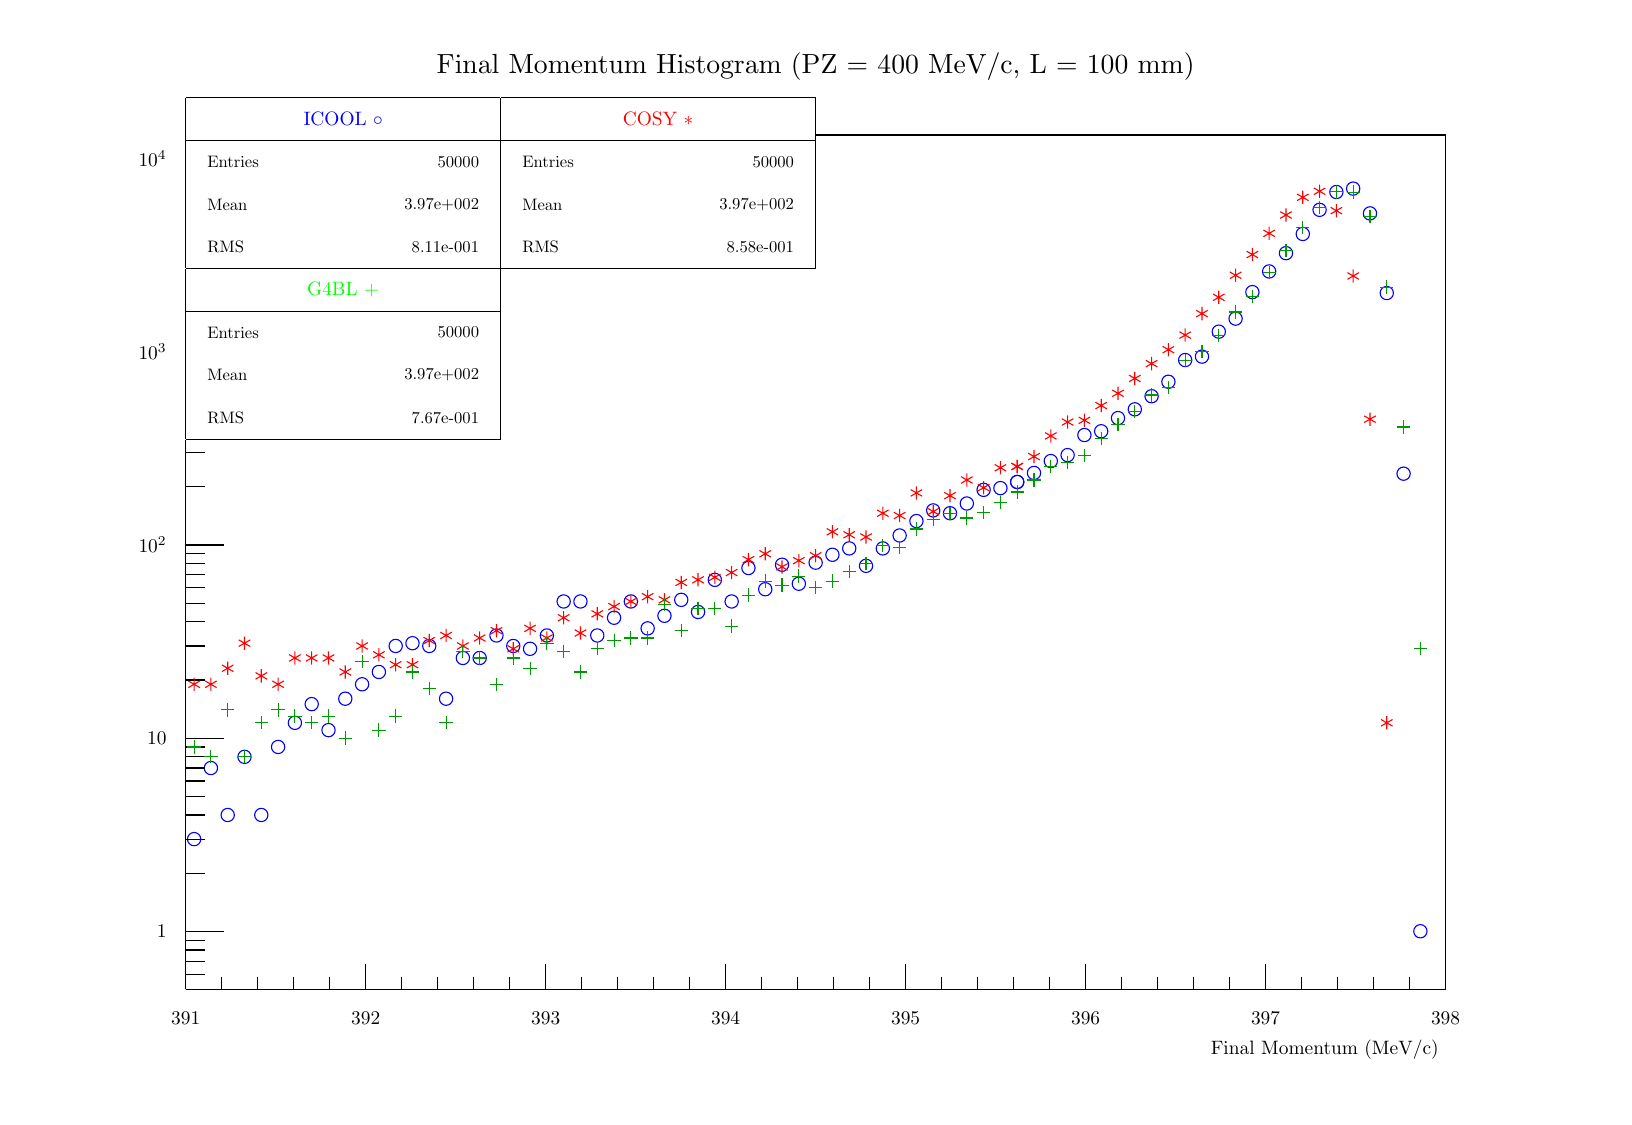
\begin{tikzpicture}
\definecolor{c}{rgb}{1,1,1};
\draw [color=c, fill=c] (0,0) rectangle (20,13.5632);
\draw [color=c, fill=c] (2,1.35632) rectangle (18,12.2069);
\definecolor{c}{rgb}{0,0,0};
\draw [c] (2,1.35632) -- (2,12.2069) -- (18,12.2069) -- (18,1.35632) -- (2,1.35632);
\definecolor{c}{rgb}{1,1,1};
\draw [color=c, fill=c] (2,1.35632) rectangle (18,12.2069);
\definecolor{c}{rgb}{0,0,0};
\draw [c] (2,1.35632) -- (2,12.2069) -- (18,12.2069) -- (18,1.35632) -- (2,1.35632);
\definecolor{c}{rgb}{0,0,1};
\foreach \P in
 {(2.10667,3.26498),(2.32,4.16755),(2.53333,3.57143),(2.74667,4.30979),(2.96,3.57143),(3.17333,4.43526),(3.38667,4.74171),(3.6,4.97941),(3.81333,4.64902),(4.02667,5.04816),(4.24,5.23123),(4.45333,5.38739),(4.66667,5.71778),(4.88,5.75271),(5.09333,5.7
1778),(5.30667,5.04816),(5.52,5.56535),(5.73333,5.56535),(5.94667,5.85111),(6.16,5.71778),(6.37333,5.68167),(6.58667,5.85111),(6.8,6.28303),(7.01333,6.28303),(7.22667,5.85111),(7.44,6.07621),(7.65333,6.28303),(7.86667,5.94118),(8.08,6.10127),(8.29333
,6.30371),(8.50667,6.1497),(8.72,6.55768),(8.93333,6.28303),(9.14667,6.70796),(9.36,6.43825),(9.57333,6.7492),(9.78667,6.50812),(10,6.77583),(10.2133,6.87617),(10.4267,6.95682),(10.64,6.73563),(10.8533,6.95682),(11.0667,7.12102),(11.28,7.30409),(11.4
933,7.4393),(11.7067,7.40343),(11.92,7.52727),(12.1333,7.70072),(12.3467,7.72257),(12.56,7.80074)}{\draw[mark options={color=c,fill=c},mark size=2.402402pt,mark=o] plot coordinates {\P};}
\foreach \P in
 {(12.56,7.80074),(12.7733,7.91498),(12.9867,8.06622),(13.2,8.1418),(13.4133,8.39687),(13.6267,8.44459),(13.84,8.61193),(14.0533,8.72323),(14.2667,8.88925),(14.48,9.07316),(14.6933,9.34913),(14.9067,9.39285),(15.12,9.7094),(15.3333,9.87504),(15.5467,
10.2115),(15.76,10.4742),(15.9733,10.7064),(16.1867,10.9502),(16.4,11.2568),(16.6133,11.483),(16.8267,11.5261),(17.04,11.2114),(17.2533,10.2),(17.4667,7.90592),(17.68,2.09469)}{\draw[mark options={color=c,fill=c},mark size=2.402402pt,mark=o] plot
 coordinates {\P};}
\definecolor{c}{rgb}{1,1,1};
\draw [color=c, fill=c] (2,10.5115) rectangle (6,12.6816);
\definecolor{c}{rgb}{0,0,0};
\draw [c] (2,10.5115) -- (6,10.5115);
\draw [c] (6,10.5115) -- (6,12.6816);
\draw [c] (6,12.6816) -- (2,12.6816);
\draw [c] (2,12.6816) -- (2,10.5115);
\draw[color=blue](4,12.4103) node[scale=0.7, rotate=0]{ICOOL $\circ$};
\draw [c] (2,12.1391) -- (6,12.1391);
\draw [anchor= west] (2.2,11.8678) node[scale=0.6, rotate=0]{Entries };
\draw [anchor= east] (5.8,11.8678) node[scale=0.6, rotate=0]{ 50000};
\draw [anchor= west] (2.2,11.3253) node[scale=0.6, rotate=0]{Mean  };
\draw [anchor= east] (5.8,11.3253) node[scale=0.6, rotate=0]{ 3.97e+002};
\draw [anchor= west] (2.2,10.7828) node[scale=0.6, rotate=0]{RMS   };
\draw [anchor= east] (5.8,10.7828) node[scale=0.6, rotate=0]{ 8.11e-001};
\draw [c] (2,1.35632) -- (18,1.35632);
\draw [anchor= east] (18,0.596782) node[scale=0.7, rotate=0]{Final Momentum (MeV/c)};
\draw [c] (2,1.68184) -- (2,1.35632);
\draw [c] (2.45714,1.51908) -- (2.45714,1.35632);
\draw [c] (2.91429,1.51908) -- (2.91429,1.35632);
\draw [c] (3.37143,1.51908) -- (3.37143,1.35632);
\draw [c] (3.82857,1.51908) -- (3.82857,1.35632);
\draw [c] (4.28571,1.68184) -- (4.28571,1.35632);
\draw [c] (4.74286,1.51908) -- (4.74286,1.35632);
\draw [c] (5.2,1.51908) -- (5.2,1.35632);
\draw [c] (5.65714,1.51908) -- (5.65714,1.35632);
\draw [c] (6.11429,1.51908) -- (6.11429,1.35632);
\draw [c] (6.57143,1.68184) -- (6.57143,1.35632);
\draw [c] (7.02857,1.51908) -- (7.02857,1.35632);
\draw [c] (7.48571,1.51908) -- (7.48571,1.35632);
\draw [c] (7.94286,1.51908) -- (7.94286,1.35632);
\draw [c] (8.4,1.51908) -- (8.4,1.35632);
\draw [c] (8.85714,1.68184) -- (8.85714,1.35632);
\draw [c] (9.31429,1.51908) -- (9.31429,1.35632);
\draw [c] (9.77143,1.51908) -- (9.77143,1.35632);
\draw [c] (10.2286,1.51908) -- (10.2286,1.35632);
\draw [c] (10.6857,1.51908) -- (10.6857,1.35632);
\draw [c] (11.1429,1.68184) -- (11.1429,1.35632);
\draw [c] (11.6,1.51908) -- (11.6,1.35632);
\draw [c] (12.0571,1.51908) -- (12.0571,1.35632);
\draw [c] (12.5143,1.51908) -- (12.5143,1.35632);
\draw [c] (12.9714,1.51908) -- (12.9714,1.35632);
\draw [c] (13.4286,1.68184) -- (13.4286,1.35632);
\draw [c] (13.8857,1.51908) -- (13.8857,1.35632);
\draw [c] (14.3429,1.51908) -- (14.3429,1.35632);
\draw [c] (14.8,1.51908) -- (14.8,1.35632);
\draw [c] (15.2571,1.51908) -- (15.2571,1.35632);
\draw [c] (15.7143,1.68184) -- (15.7143,1.35632);
\draw [c] (16.1714,1.51908) -- (16.1714,1.35632);
\draw [c] (16.6286,1.51908) -- (16.6286,1.35632);
\draw [c] (17.0857,1.51908) -- (17.0857,1.35632);
\draw [c] (17.5429,1.51908) -- (17.5429,1.35632);
\draw [c] (18,1.68184) -- (18,1.35632);
\draw [anchor=base] (2,0.908736) node[scale=0.7, rotate=0]{391};
\draw [anchor=base] (4.28571,0.908736) node[scale=0.7, rotate=0]{392};
\draw [anchor=base] (6.57143,0.908736) node[scale=0.7, rotate=0]{393};
\draw [anchor=base] (8.85714,0.908736) node[scale=0.7, rotate=0]{394};
\draw [anchor=base] (11.1429,0.908736) node[scale=0.7, rotate=0]{395};
\draw [anchor=base] (13.4286,0.908736) node[scale=0.7, rotate=0]{396};
\draw [anchor=base] (15.7143,0.908736) node[scale=0.7, rotate=0]{397};
\draw [anchor=base] (18,0.908736) node[scale=0.7, rotate=0]{398};
\draw [c] (2,1.35632) -- (2,12.2069);
\draw [c] (2.24,1.35632) -- (2,1.35632);
\draw [c] (2.24,1.55054) -- (2,1.55054);
\draw [c] (2.24,1.71475) -- (2,1.71475);
\draw [c] (2.24,1.85699) -- (2,1.85699);
\draw [c] (2.24,1.98246) -- (2,1.98246);
\draw [c] (2.48,2.09469) -- (2,2.09469);
\draw [anchor= east] (1.844,2.09469) node[scale=0.7, rotate=0]{1};
\draw [c] (2.24,2.83306) -- (2,2.83306);
\draw [c] (2.24,3.26498) -- (2,3.26498);
\draw [c] (2.24,3.57143) -- (2,3.57143);
\draw [c] (2.24,3.80913) -- (2,3.80913);
\draw [c] (2.24,4.00335) -- (2,4.00335);
\draw [c] (2.24,4.16755) -- (2,4.16755);
\draw [c] (2.24,4.3098) -- (2,4.3098);
\draw [c] (2.24,4.43526) -- (2,4.43526);
\draw [c] (2.48,4.5475) -- (2,4.5475);
\draw [anchor= east] (1.844,4.5475) node[scale=0.7, rotate=0]{10};
\draw [c] (2.24,5.28587) -- (2,5.28587);
\draw [c] (2.24,5.71778) -- (2,5.71778);
\draw [c] (2.24,6.02423) -- (2,6.02423);
\draw [c] (2.24,6.26194) -- (2,6.26194);
\draw [c] (2.24,6.45615) -- (2,6.45615);
\draw [c] (2.24,6.62036) -- (2,6.62036);
\draw [c] (2.24,6.7626) -- (2,6.7626);
\draw [c] (2.24,6.88807) -- (2,6.88807);
\draw [c] (2.48,7.0003) -- (2,7.0003);
\draw [anchor= east] (1.844,7.0003) node[scale=0.7, rotate=0]{$10^{2}$};
\draw [c] (2.24,7.73867) -- (2,7.73867);
\draw [c] (2.24,8.17059) -- (2,8.17059);
\draw [c] (2.24,8.47704) -- (2,8.47704);
\draw [c] (2.24,8.71474) -- (2,8.71474);
\draw [c] (2.24,8.90896) -- (2,8.90896);
\draw [c] (2.24,9.07316) -- (2,9.07316);
\draw [c] (2.24,9.21541) -- (2,9.21541);
\draw [c] (2.24,9.34087) -- (2,9.34087);
\draw [c] (2.48,9.45311) -- (2,9.45311);
\draw [anchor= east] (1.844,9.45311) node[scale=0.7, rotate=0]{$10^{3}$};
\draw [c] (2.24,10.1915) -- (2,10.1915);
\draw [c] (2.24,10.6234) -- (2,10.6234);
\draw [c] (2.24,10.9298) -- (2,10.9298);
\draw [c] (2.24,11.1675) -- (2,11.1675);
\draw [c] (2.24,11.3618) -- (2,11.3618);
\draw [c] (2.24,11.526) -- (2,11.526);
\draw [c] (2.24,11.6682) -- (2,11.6682);
\draw [c] (2.24,11.7937) -- (2,11.7937);
\draw [c] (2.48,11.9059) -- (2,11.9059);
\draw [anchor= east] (1.844,11.9059) node[scale=0.7, rotate=0]{$10^{4}$};
\definecolor{c}{rgb}{1,1,1};
\draw [color=c, fill=c] (2,10.5115) rectangle (6,12.6816);
\definecolor{c}{rgb}{0,0,0};
\draw [c] (2,10.5115) -- (6,10.5115);
\draw [c] (6,10.5115) -- (6,12.6816);
\draw [c] (6,12.6816) -- (2,12.6816);
\draw [c] (2,12.6816) -- (2,10.5115);
\draw[color=blue](4,12.4103) node[scale=0.7, rotate=0]{ICOOL $\circ$};
\draw [c] (2,12.1391) -- (6,12.1391);
\draw [anchor= west] (2.2,11.8678) node[scale=0.6, rotate=0]{Entries };
\draw [anchor= east] (5.8,11.8678) node[scale=0.6, rotate=0]{ 50000};
\draw [anchor= west] (2.2,11.3253) node[scale=0.6, rotate=0]{Mean  };
\draw [anchor= east] (5.8,11.3253) node[scale=0.6, rotate=0]{ 3.97e+002};
\draw [anchor= west] (2.2,10.7828) node[scale=0.6, rotate=0]{RMS   };
\draw [anchor= east] (5.8,10.7828) node[scale=0.6, rotate=0]{ 8.11e-001};
\draw (10,13.0816) node[scale=1, rotate=0]{Final Momentum Histogram (PZ = 400 MeV/c, L = 100 mm)};
\definecolor{c}{rgb}{1,0,0};
\foreach \P in
 {(2.10667,5.23123),(2.32,5.23123),(2.53333,5.43474),(2.74667,5.75271),(2.96,5.33784),(3.17333,5.23123),(3.38667,5.56535),(3.6,5.56535),(3.81333,5.56535),(4.02667,5.38739),(4.24,5.71778),(4.45333,5.60555),(4.66667,5.48008),(4.88,5.48008),(5.09333,5.7
8653),(5.30667,5.85111),(5.52,5.71778),(5.73333,5.81931),(5.94667,5.912),(6.16,5.68167),(6.37333,5.94118),(6.58667,5.81931),(6.8,6.07621),(7.01333,5.88199),(7.22667,6.12576),(7.44,6.21845),(7.65333,6.28303),(7.86667,6.34392),(8.08,6.30371),(8.29333,6
.5249),(8.50667,6.55768),(8.72,6.58948),(8.93333,6.65037),(9.14667,6.81457),(9.36,6.88807),(9.57333,6.72189),(9.78667,6.80182),(10,6.86413),(10.2133,7.16755),(10.4267,7.13049),(10.64,7.10183),(10.8533,7.40343),(11.0667,7.37384),(11.28,7.66137),(11.49
33,7.4251),(11.7067,7.62644),(11.92,7.82557),(12.1333,7.72796),(12.3467,7.98062),(12.56,7.99747)}{\draw[mark options={color=c,fill=c},mark size=2.402402pt,mark=asterisk] plot coordinates {\P};}
\foreach \P in
 {(12.56,7.99747),(12.7733,8.1234),(12.9867,8.38532),(13.2,8.56148),(13.4133,8.5834),(13.6267,8.77076),(13.84,8.92656),(14.0533,9.11494),(14.2667,9.30354),(14.48,9.48045),(14.6933,9.66581),(14.9067,9.93835),(15.12,10.1458),(15.3333,10.4253),(15.5467,
10.6888),(15.76,10.958),(15.9733,11.1909),(16.1867,11.4156),(16.4,11.4924),(16.6133,11.246),(16.8267,10.4167),(17.04,8.59776),(17.2533,4.74171)}{\draw[mark options={color=c,fill=c},mark size=2.402402pt,mark=asterisk] plot coordinates {\P};}
\definecolor{c}{rgb}{1,1,1};
\draw [color=c, fill=c] (6,10.5115) rectangle (10,12.6816);
\definecolor{c}{rgb}{0,0,0};
\draw [c] (6,10.5115) -- (10,10.5115);
\draw [c] (10,10.5115) -- (10,12.6816);
\draw [c] (10,12.6816) -- (6,12.6816);
\draw [c] (6,12.6816) -- (6,10.5115);
\draw [color=red](8,12.4103) node[scale=0.7, rotate=0]{COSY $*$};
\draw [c] (6,12.1391) -- (10,12.1391);
\draw [anchor= west] (6.2,11.8678) node[scale=0.6, rotate=0]{Entries };
\draw [anchor= east] (9.8,11.8678) node[scale=0.6, rotate=0]{ 50000};
\draw [anchor= west] (6.2,11.3253) node[scale=0.6, rotate=0]{Mean  };
\draw [anchor= east] (9.8,11.3253) node[scale=0.6, rotate=0]{ 3.97e+002};
\draw [anchor= west] (6.2,10.7828) node[scale=0.6, rotate=0]{RMS   };
\draw [anchor= east] (9.8,10.7828) node[scale=0.6, rotate=0]{ 8.58e-001};
\definecolor{c}{rgb}{1,1,1};
\draw [color=c, fill=c] (6,10.5115) rectangle (10,12.6816);
\definecolor{c}{rgb}{0,0,0};
\draw [c] (6,10.5115) -- (10,10.5115);
\draw [c] (10,10.5115) -- (10,12.6816);
\draw [c] (10,12.6816) -- (6,12.6816);
\draw [c] (6,12.6816) -- (6,10.5115);
\draw [color=red](8,12.4103) node[scale=0.7, rotate=0]{COSY $*$};
\draw [c] (6,12.1391) -- (10,12.1391);
\draw [anchor= west] (6.2,11.8678) node[scale=0.6, rotate=0]{Entries };
\draw [anchor= east] (9.8,11.8678) node[scale=0.6, rotate=0]{ 50000};
\draw [anchor= west] (6.2,11.3253) node[scale=0.6, rotate=0]{Mean  };
\draw [anchor= east] (9.8,11.3253) node[scale=0.6, rotate=0]{ 3.97e+002};
\draw [anchor= west] (6.2,10.7828) node[scale=0.6, rotate=0]{RMS   };
\draw [anchor= east] (9.8,10.7828) node[scale=0.6, rotate=0]{ 8.58e-001};
\definecolor{c}{rgb}{0,0.6,0};
\foreach \P in
 {(2.10667,4.43526),(2.32,4.30979),(2.53333,4.90592),(2.74667,4.30979),(2.96,4.74171),(3.17333,4.90592),(3.38667,4.82698),(3.6,4.74171),(3.81333,4.82698),(4.02667,4.5475),(4.24,5.52357),(4.45333,4.64902),(4.66667,4.82698),(4.88,5.38739),(5.09333,5.17
363),(5.30667,4.74171),(5.52,5.64429),(5.73333,5.56535),(5.94667,5.23123),(6.16,5.56535),(6.37333,5.43474),(6.58667,5.75271),(6.8,5.64429),(7.01333,5.38739),(7.22667,5.68167),(7.44,5.78653),(7.65333,5.81931),(7.86667,5.81931),(8.08,6.24041),(8.29333,
5.912),(8.50667,6.19602),(8.72,6.19602),(8.93333,5.96959),(9.14667,6.36346),(9.36,6.54142),(9.57333,6.49108),(9.78667,6.60503),(10,6.45615),(10.2133,6.54142),(10.4267,6.66506),(10.64,6.7626),(10.8533,6.9896),(11.0667,6.96786),(11.28,7.20336),(11.4933
,7.31999),(11.7067,7.39611),(11.92,7.3434),(12.1333,7.4107),(12.3467,7.54018),(12.56,7.67276)}{\draw[mark options={color=c,fill=c},mark size=2.402402pt,mark=+] plot coordinates {\P};}
\foreach \P in
 {(12.56,7.67276),(12.7733,7.82557),(12.9867,7.99747),(13.2,8.04645),(13.4133,8.13814),(13.6267,8.34991),(13.84,8.53407),(14.0533,8.69539),(14.2667,8.9054),(14.48,9.00076),(14.6933,9.33969),(14.9067,9.45948),(15.12,9.66056),(15.3333,9.95909),(15.5467
,10.1596),(15.76,10.459),(15.9733,10.7368),(16.1867,11.0367),(16.4,11.2896),(16.6133,11.4844),(16.8267,11.4817),(17.04,11.172),(17.2533,10.2749),(17.4667,8.49813),(17.68,5.68167)}{\draw[mark options={color=c,fill=c},mark size=2.402402pt,mark=+] plot
 coordinates {\P};}
\definecolor{c}{rgb}{1,1,1};
\draw [color=c, fill=c] (2,8.34138) rectangle (6,10.5115);
\definecolor{c}{rgb}{0,0,0};
\draw [c] (2,8.34138) -- (6,8.34138);
\draw [c] (6,8.34138) -- (6,10.5115);
\draw [c] (6,10.5115) -- (2,10.5115);
\draw [c] (2,10.5115) -- (2,8.34138);
\draw [color=green](4,10.2402) node[scale=0.7, rotate=0]{G4BL $+$};
\draw [c] (2,9.96897) -- (6,9.96897);
\draw [anchor= west] (2.2,9.6977) node[scale=0.6, rotate=0]{Entries };
\draw [anchor= east] (5.8,9.6977) node[scale=0.6, rotate=0]{ 50000};
\draw [anchor= west] (2.2,9.15517) node[scale=0.6, rotate=0]{Mean  };
\draw [anchor= east] (5.8,9.15517) node[scale=0.6, rotate=0]{ 3.97e+002};
\draw [anchor= west] (2.2,8.61264) node[scale=0.6, rotate=0]{RMS   };
\draw [anchor= east] (5.8,8.61264) node[scale=0.6, rotate=0]{ 7.67e-001};
\definecolor{c}{rgb}{1,1,1};
\draw [color=c, fill=c] (2,8.34138) rectangle (6,10.5115);
\definecolor{c}{rgb}{0,0,0};
\draw [c] (2,8.34138) -- (6,8.34138);
\draw [c] (6,8.34138) -- (6,10.5115);
\draw [c] (6,10.5115) -- (2,10.5115);
\draw [c] (2,10.5115) -- (2,8.34138);
\draw [color=green](4,10.2402) node[scale=0.7, rotate=0]{G4BL $+$};
\draw [c] (2,9.96897) -- (6,9.96897);
\draw [anchor= west] (2.2,9.6977) node[scale=0.6, rotate=0]{Entries };
\draw [anchor= east] (5.8,9.6977) node[scale=0.6, rotate=0]{ 50000};
\draw [anchor= west] (2.2,9.15517) node[scale=0.6, rotate=0]{Mean  };
\draw [anchor= east] (5.8,9.15517) node[scale=0.6, rotate=0]{ 3.97e+002};
\draw [anchor= west] (2.2,8.61264) node[scale=0.6, rotate=0]{RMS   };
\draw [anchor= east] (5.8,8.61264) node[scale=0.6, rotate=0]{ 7.67e-001};
\end{tikzpicture}
